\documentclass[a4paper,norsk]{article}
\usepackage{preamble}


\usepackage{color, colortbl}
\definecolor{LightCyan}{rgb}{0.88,1,1}


\begin{document}
\maketitle
\section*{Taylor-Green Vortex}


\section*{Physical problem}
The Taylor-Green vortex is a unsteady flow were we observe the flow of a decaying
vortex. This flow has an exact solution for the incrompessible Navier-Stokes equation in 2D, while for the 3D
case there are several numerical results for comparison.
Assuming the fluid is incompressible, the exact solution for velocity and pressure are given as ($t=0$)

\begin{align}
u(x,y,t) = (V_{0} cos(\pi x)sin(\pi y) e^{-2 t \nu \pi^{2} }, \hspace{2mm} V_{0}cos(\pi y)sin(\pi x) e^{-2 t \nu \pi^2} ) \\
p(x,y,t) = -0.25(cos(2\pi x) + cos(2 \pi y) ) e^{-4 t \nu \pi^2}
\end{align}


For the 3D case we will consider the kinetic energy $E_k$ and kinetic energy dissipation rate $\epsilon$  for the system. These quantities are
explored thoroughly by other authors, and will be used as comparison. The initial field set up in the 3D Taylor-Green vortex is defined as

\begin{align}
u(x,y,z) = ( V_{0}sin(\frac{x}{L}) cos(\frac{y}{L}) cos(\frac{z}{L}), \hspace{2mm}-V_{0}cos(\frac{x}{L})sin(\frac{y}{L})cos(\frac{z}{L}), \hspace{2mm} 0 )\\
p(x,y,z) = \rho_{0} + \frac{\rho_0 V_0^2}{16}(cos(\frac{2x}{L}) + cos(\frac{2y}{L}))(cos(\frac{2z}{L}) + 2)
\end{align}

Exploring the incompressible flow condition we define $\rho_0 = \rho$, and for simplicity we let $V_0 = 1$

\section*{Governing Equation and Computations}
The incompressible Naiver-Stokes equation describes the flow motion, from the principles of conservation of momentum
and continuum.

\begin{align}
&\frac{\partial \textbf{v}}{\partial t} + \textbf{v} \cdot \nabla \textbf{v} =
-\nabla p + \nu \nabla^2 \textbf{v} \\
&\nabla \cdot \textbf{v} = 0
\end{align}

There is a open sea full of different approaches to solve this non-linear equation. We will for this
time explore Chorins method, and the incremental pressure correction scheme (\textit{IPCS}).

We will use the FEniCS project, a open-source PDE solver using the finite element method approach.
As verification of our schemes, the known analytical solution for the 2D Taylor-Green Vortex will be used as comparison.
Finally we will move on to the 3D Taylor-Green vortex, using ... as reference.

The Reynolds number, discovered Osborne Reynolds as the relation between inertial and viscous forces, is defined
as
\begin{align}
Re = \frac{\rho V_{0} L}{\mu} = \frac{V_{0} L}{\nu}
\end{align}
Where $\nu$ denotes the kinematic viscosity, while $U_{0}$ and \textit{D} is some characteristic velocity and lenght.

We define the kinetic energy as $E_k = \frac{1}{2}||u||^2_{L^2}$, and the kinetic energy dissipation rate $\epsilon = \frac{-d E_k}{dt}$

\newpage
\section*{Setting up 2D problem}

For the 2D case, the computational domain is set as $\Omega \in [-1, 1]^2$. Further on we will set
the flow conditions as \\

\begin{tabular}{l*{6}{c}r}
Physical Quantity              & Value  \\
\hline
Reynolds Number, Re & 1000   \\
Characteristic length, L           & 2     \\
Characteristic velocity, $V_{0}$   & 1     \\
Space discretization, N & [8, 16, 32, 64] \\
Time step $\Delta t$ 			   & [0.1, 0.01, 0.001] \\
End time, T 					   & 1.0
\end{tabular}

Using our analytical solution for time $t = 0$, we set up the initial condition
for the domain $\Omega$

\begin{figure}[h!]
	\centering
	\caption*{Initial velocity field}
	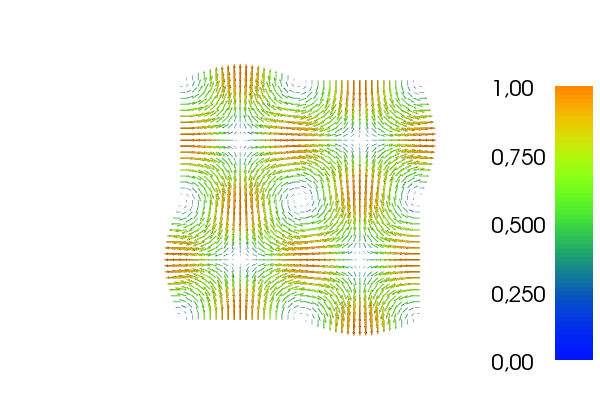
\includegraphics[scale=0.32]{2D/initial.png}
    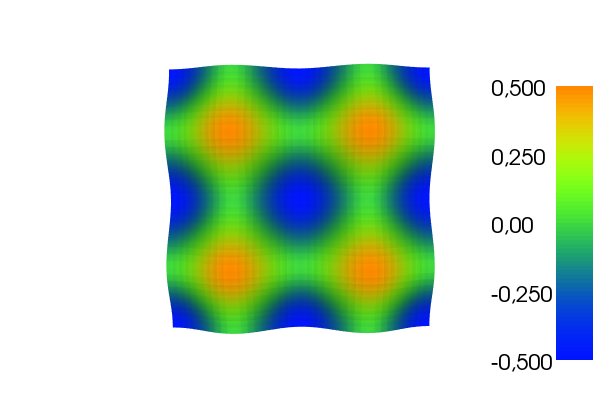
\includegraphics[scale=0.32]{2D/initpress.png}
\end{figure}


\section*{Results}
Experiments run for Time $T = 1$ for different choices of dt and N

\textit{IPCS}
\begin{table}[ht]
\centering
\begin{tabular}{c|ccccccc}
\hline
\rowcolor{LightCyan}
N  &  $L_2$ dt = 0.1 & Runtime & $L_2$ dt = 0.01 & Runtime  & $L_2$ dt = 0.001  & Runtime\\
\hline
8  & 0.721623  & 0.410195 & 0.180146    & 0.652783 & 0.178604    & 3.73357 \\ \hline
\rowcolor{LightCyan}
16 & 5.34035   & 0.171748 & 0.0184505   & 0.871824 & 0.0184569   & 6.47402 \\ \hline
32 & 0.321217  & 0.361791 & 0.00122458  & 1.90135  & 0.00122848  & 17.9395 \\ \hline
\rowcolor{LightCyan}
64 & 0.0046837 & 1.11411  & 0.000913817 & 6.26709  & 0.000103177 & 62.2844 \\
\hline
\end{tabular}
\end{table}

\textit{Chorin}

\begin{table}[ht]
\centering
\begin{tabular}{c|ccccccc}
\hline
\rowcolor{LightCyan}
N  &  $L_2$ dt = 0.1 & Runtime & $L_2$ dt = 0.01 & Runtime  & $L_2$ dt = 0.001  & Runtime\\
\hline
8  & 0.840517   & 1.382    & 0.210405    & 0.382298 & 0.201774    & 3.26483 \\ \hline
\rowcolor{LightCyan}
16 & 4.81879    & 0.173606 & 0.0314729   & 0.698007 & 0.0292556   & 6.25138 \\ \hline
32 & 0.0543076  & 0.342292 & 0.00307992  & 1.78643  & 0.00226862  & 16.8787 \\ \hline
\rowcolor{LightCyan}
64 & 0.00329629 & 1.16073  & 0.000444121 & 6.02408  & 0.000178841 & 71.846 \\ 
\hline
\end{tabular}
\end{table}

\newpage
\section*{Setting up 3D problem}
The computational domain is defined as a cube with sides of length $2 \pi L$, $-\pi L \leq x,y,z \leq \pi L$. We set our 
physical quantities as follows. 

\begin{tabular}{l*{6}{c}r}
Physical Quantity              & Value  \\
\hline
Reynolds Number, Re & 1000   \\
Characteristic length, L           & 1     \\
Characteristic velocity, $V_{0}$   & 1     \\
Time step $\Delta t$ 			   & 0.001 \\
End time, T 					   & 10.0
\end{tabular}
Further exploration in the coarseness of the discretization in space and time will be investigated aswell.

\newpage
\section*{Results and Comments}
\begin{table}[h!]
\centering
\begin{tabular}{c|ccc}
\hline
\rowcolor{LightCyan}
Solver  &  Chorin & IPCS & Oasis\\
\hline
Computer & Abel    & Abel & Enkidu    \\ \hline
\rowcolor{LightCyan}
Simulaton hours & 11.14  & 9.30 & INFO  \\ \hline
Cores & 3 & 3  & 1  \\ \hline
\rowcolor{LightCyan}
Elements &P2-P1 & P2-P1 & P2-P1 \\ \hline
DOF V & 786432 & 786432 & INFO \\ \hline
\rowcolor{LightCyan}
DOF P & 32768 &  32768 & INFO \\
\hline
\end{tabular}
\end{table}

\begin{figure}[h!]
	\centering
	%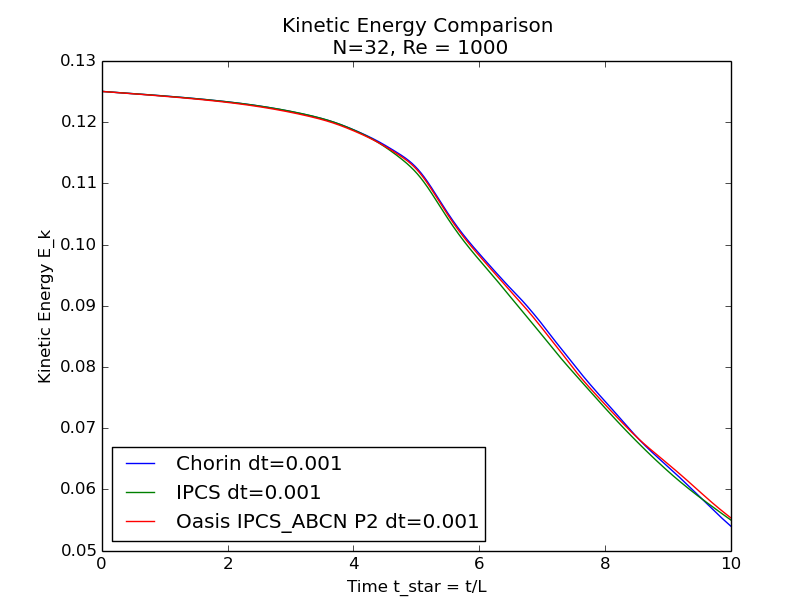
\includegraphics[scale=0.5]{results/plots/Ek_dt001.png}
    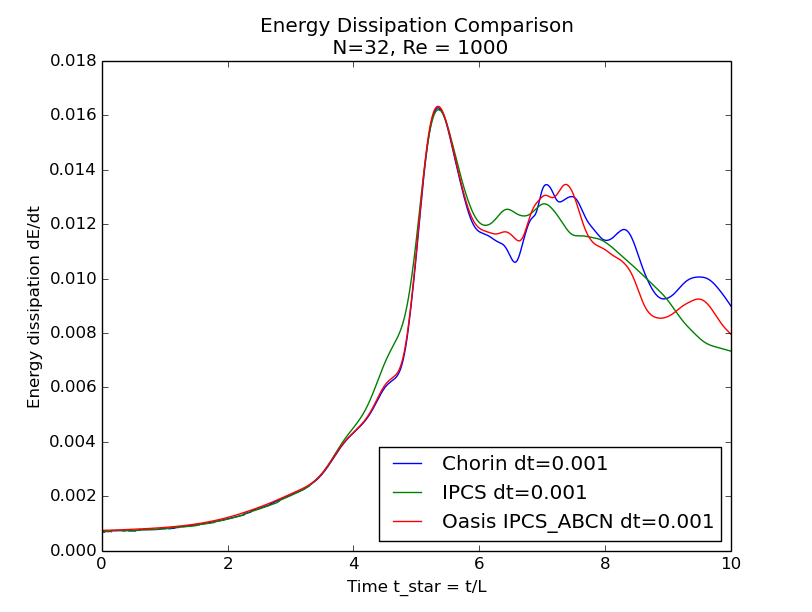
\includegraphics[scale=0.5]{results/plots/dkdt_dt001.png}
\end{figure}

Our numerical computations yields some interesting results. Tracking the energy dissipation towards the distinctive top at $t \approx 5.8 s$, we observe a small deviation in the IPCS solver in the time domain $t = [4, 5]$. Apart from this this time domain, the solvers match the Oasis computations rather good. Continuing downhill after the distinctive top, the solvers deviate from another at $t = \approx 6 s$. We observe that the initial vortexes at this points gets highly turbulent as the energy within the fluid is driven into smaller vortices. According to the Oasis solver, it seems that my implementations are not able to "catch" all of the fluctuations within the fluid.
\\ \\
\newpage
\begin{figure}[h!]
	\centering
	\caption*{Chorin comparison of dt = [0.01, 0.001]}
	%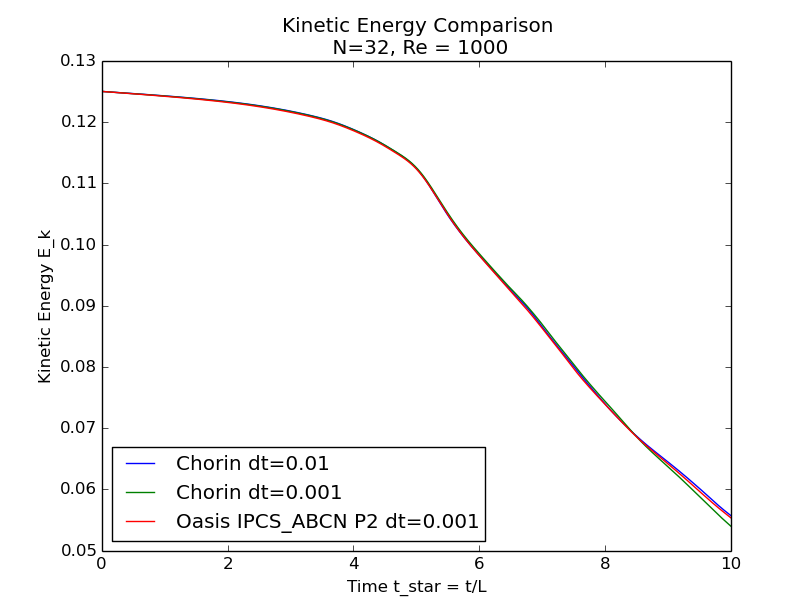
\includegraphics[scale=0.37]{results/plots/chorin_comp.png}
    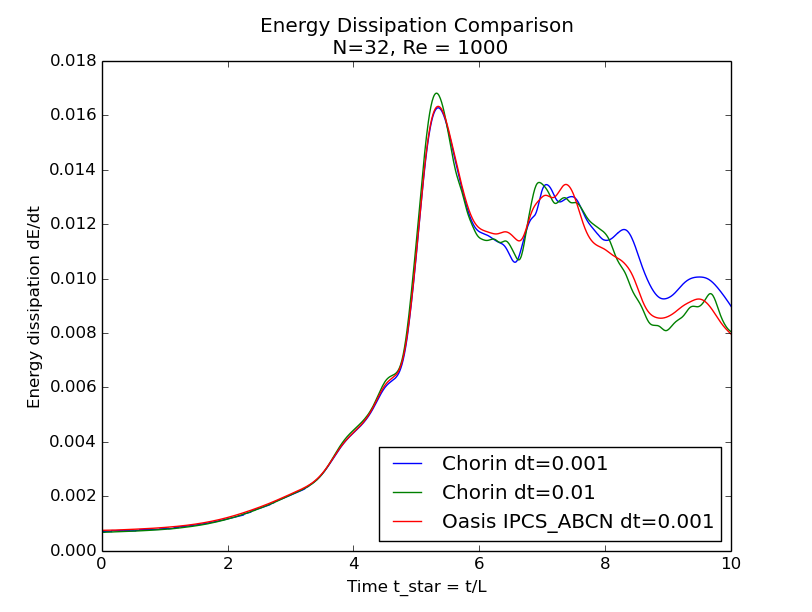
\includegraphics[scale=0.5]{results/plots/chorin_comp2.png}
\end{figure}
\begin{figure}[h!]
	\centering
	\caption*{IPCS comparison of dt = [0.01, 0.001]}
    %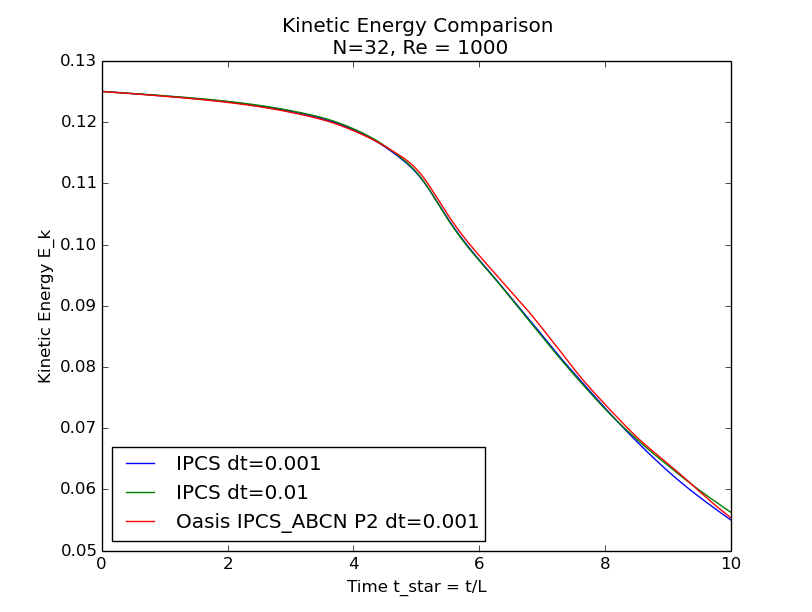
\includegraphics[scale=0.34]{results/plots/ipcs_comp.png}
    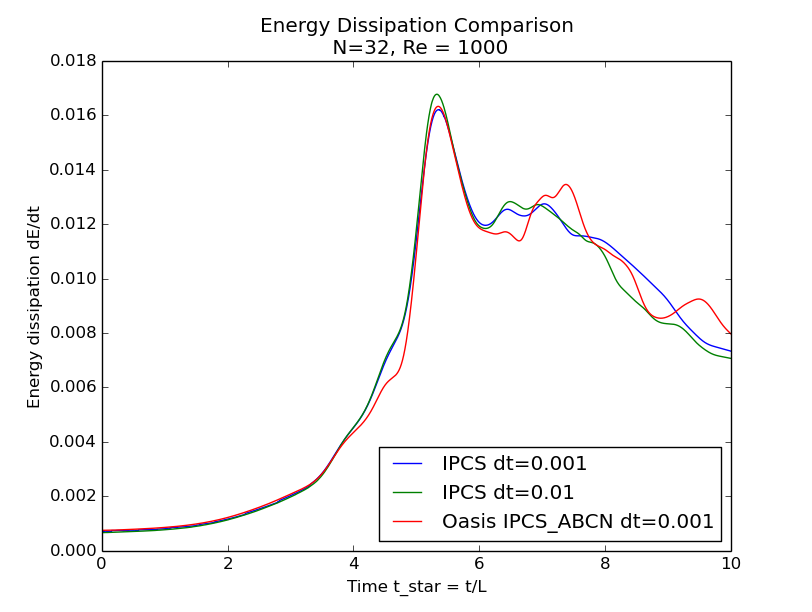
\includegraphics[scale=0.5]{results/plots/ipcs_comp2.png}
\end{figure}

Moving on to comparing coarseness of the time discretization, we compared $dt = 0.01, 0.1$ for both solvers. The case of
$dt = 0.1$ diverged after fairly few steps for both solvers. Due to the high Reynolds number chosen for this case, the solvers can't intercept all the fluctuations within the fluid for such a large choice of dt. For the $dt = 0.01$ experiment, we observe that the data cling on the finer discretization in time $dt = 0.001$ fairly well upon reaching the distinctive top in the energy dissipation plot. Here both solvers seems to overestimate the dissipation peak. before falling in with the finer discretization towards the separation point from the Oasis solver at $t \approx 6$, which we mentioned in the main experiment. 
\newpage
For the coarseness of the space discretization, comparisons between $N = 16, 32, 64$ where tried out. For the $N = 16$ case, the numerical calculations also diverged.....Venter på data

\end{document}
